% !TEX encoding = UTF-8
% !TEX program = pdflatex

\documentclass[a4paper]{report}
\usepackage[T1]{fontenc}
\usepackage[utf8]{inputenc}
\usepackage[english]{babel}
\usepackage{graphicx}

\begin{document}

\begin{titlepage}
\centering
\vspace*{\stretch{1}}

\includegraphics{logoRomaTre.jpg}\\
\vspace*{\stretch{6}}
{\LARGE \bf Web Services Platform for the visualization of gene expression data\par}
\vspace{0.5cm}
{\Large Comparison between experiments and differential analysis\par} 
\vspace{2cm}
di\\
{\Large \em Chiara Bartalotta, Dario Santilli, Davide Bernardini\par}
\vspace*{\stretch{2}}
\date{\currenttime}
\today
\end{titlepage}

\begin{Large}
Un po di cose riguardo il progetto, romatre e l'istituto.\\
\end{Large}

\tableofcontents

\part{Introduction}
\chapter{Gene Expression}
\section{prima sezione}
\begin{figure}[b]
\centering

\includegraphics[height=5.5cm, width=11.5cm]{logoRomaTre.jpg}
\end{figure}
Varie cose
\begin{itemize}
    \item \textbf{uno}: unopuntouno;
    \item \textbf{due}: ecc;
    \item \textbf{tre}: ecc.
\end{itemize}
inserire frase.\\
e un'altra... \\
..e un'altra. \\

\section{Talk About the Institute C.S.S. Mendel?}
Facciamo di sì.\\
\\\\\\
..images testing..
\begin{figure}[h]
\centering

\includegraphics[height=12cm, width=6cm]{logoRomaTre.jpg}
\end{figure}

\begin{figure}[hb]
\centering

\includegraphics[height=3cm, width=6cm]{logoRomaTre.jpg}
\end{figure}

\chapter{Main features of the project}
\section{Aims}


\section{Function and structure}
The portal is used by two types of users:
\begin{itemize}
   \item \textit{super user}: VIP;
   \item \textit{simple user}: others;
\end{itemize}

-STRUTTURA GENERALE (scrivere alla fine)-


\section{Tools}
bla,bla,bla



\chapter{Technologies}
WEB-gene expression is developed as a web platform following the guide of the client-server architecture. The platform was built using JavaScript and jQuery to manage the client-side and the html page, and php and MySQL to manage the server-side. This chapter provides a description of these technologies and an explanation about how these technologies were used.

\section{Client-Server Architecture}

The Client-Server Architecture is a structure adopted to develop software applications. The objective of the Client-Server model is to divide the tasks of the application between the server and the client. The work of the Client is to request a service to a server which provides functions in order to respond to the request of the Client.\\
The browser is an example of Client. The browser connects itself to a Server that provides the information required by the user. In this way, the browser displays the response allowing the user to interact with this information. The program that responds to the browser request is an example of Server. It is listening to client requests, and it is always ready to provide the response.\\
The Figure \ref{clientServer} is a computer network diagram that shows the communication between clients and server by internet. In the figure, two clients are represented in order to indicate that the server receives the requests from multiple clients as described in section \ref{serverside}. 

\begin{figure}[htb] 
\begin{center}
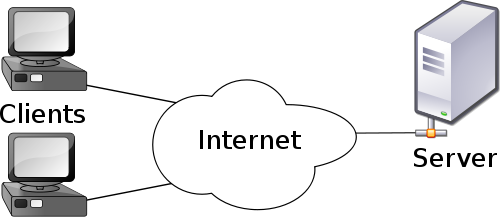
\includegraphics[scale=0.4]{figure/clientServer.png} 
\end{center}
\caption{Client-Server architecture.}
\label{clientServer}
\end{figure}

\subsection{Communication Protocol}

The Client side and the Server Side exchange message between each other using a Communication Protocol. A communication protocol defines rules about the syntax, the semantic and the synchronization of communication in order to manage the message exchange among computer systems.  Each message has a defined format, and its objective is to provoke a specific response from the receiver.

\\In WEB-gene-expression, the server side and the client side communicate through the HTTP protocol (HyperText Transfer Protocol) that is based on TCP/IP (Transmission Control Protocol / Internet Protocol). This protocol allows the server side and the client side to exchange ordered byte sequences.
\\In order to access the resource, the client side sends the server side a string of characters defined as URI (Uniform Resource Identifier). Each URI refers to a specific resource.

\subsection{Sever-Side}\label{serverside}

The server is always listening to the requests of the Clients. When a requests arrives, the Server provides the response by running an application able to satisfy the Client request.\\
The Server is able to satisfy many requests coming from different clients at the same time.\\
With regards to WEB-gene-expression, php is the language used to develop the server side. The framework adopted to create the web application in PHP is XAMPP.


\subsubsection{Server Tasks} 
In WEB-gene-expression, the server side has the task to manage the client requests by connecting the system to the database and providing the response data. \\
The database guarantees the data persistence while the server side organizes the application logic for managing of the operations with the data.\\

\subsubsection{The PHP language}\label{php}

The programming language used to develop the server side of WEB-gene-expression is PHP. 

\\"PHP is a popular general-purpose scripting language that is especially suited to web development. Fast, flexible and pragmatic, PHP powers everything from your blog to the most popular websites in the world." \footnote{www.php.net}


Therefore, the main features of PHP meet WEB-gene-expression requirements for the implementation of the server side. The code is organized in classes following the principles of \emph{High Cohesion} and \emph{Low Coupling} described in "Applicare UML e i pattern" \footcite{Craig Larman, Luca Cabibbo} . \\
The \emph{Low Coupling} pattern describes how to keep a low dependency among objects in order to guarantee a better usability of the code and a lower impact of the code changes.\\
The \emph{High Cohesion} pattern describes how to assign a specific, focused and comprehensible responsibility to each object in order to provide maintainability of the code.\\

\subsubsection{XAMPP}

XAMPP is an usefull environment for development of web applications in PHP. XAMPP aims at offering intuitive tools that allow the developer to create pure PHP web applications in a fast way \footnote{https://www.apachefriends.org/index.html}.\\
XAMPP is used to develop the server-side of WEB-gene-expression and his distribution contains not only PHP but also MySQL database.

\subsection{Database}

The database is responsible of information persistence. WEB-gene-application has to operate a large amount of data coming from the experiment about differential analysis of gene expression data. In order to store these data, SICS use \emph{MySQL} as database.

\subsubsection{MySQL}

MySQL\footnote{http://www.mysql.it/} is a powerful, open source object-relational database system that runs on all major operating systems.
\\During the development phase, MySQL was chosen as WEB-gene-expression database for the following features. MySQL guarantees reliability, data integrity, correctness and stability. Furthermore, the extensible features and the large compatibility of MySQL are key features required by WEB-gene-expression. Due to these characteristics, WEB-gene-expression can be efficiently extend and reused in other systems.

\subsubsection{DataBase structure}

In an entity-relation database, the information is organized in different tables connected between each other through relations. Each table represents a concept of an entity and contains the instances of this entity. The \emph{entities} describe classes of objects with common properties but autonomous existence. The \emph{relations} represent the logic links between two or more entities.\\
The database in SICS is composed of five table which represent the entities of the application. \emph{Experiments} table collects the instances saved by the super user. It contains an univocal id, the name of the item, the date corresponding at the time when the experiment was loaded. The \emph{Analysis} table stores the differential analysis of an experiment. His columns are	univocal id, geneSymbol on which the analysis is done, p\_value , foldChange, the name of the analysis, the date an the id of the corresponding experiment. 
The \emph{Gene} table collects information about genes. This information are 	univocal id, geneSymbol, geneAssignment and refSeq.
\emph{Users} table collects the data regarding the users of the system. Each record contains the univocal id,name, surname, email, password and type of an user.
 Finally, the last table is the \emph{View Permission} table that collects the permissions of each user. With the two columns , id user and id experiment, this table stores the experiments that a normal user can visualize.\\

\paragraph{}The following logic schema describes the entity tables:
\begin{quote}
\item EXPERIMENT(\underline{id}, name, date) 
\item ANALYSIS(\underline{id}, geneSymbol, p\_value, foldChange, name, date, id\_experiment) with referential integrity between the \emph{id\_experiment} attribute and the \emph{EXPERIMENT} relation and between the \emph{geneSymbol} attribute and the \emph{GENE} relation.
\item GENE(\underline{id}, geneSymbol, geneAssignment, refSeq) 
\item USER(\underline{id}, name, surname, email, password, type) 
\item VIEWPERMISSION(\underline{id\_user}, \underline{id\_experiment})  with referential integrity between the \emph{id\_user} attribute and the \emph{USER} relation and between the \emph{id\_experiment} attribute and the \emph{EXPERIMENTS} relation.
\end{quote}

\subsubsection{JavaScript and jQuery}

\paragraph{JavaScript}
JavaScript is considered the most appropriate language for development of web applications.
 ``JavaScript is a lightweight, interpreted, object-oriented language with first-class functions, most known as the scripting language for Web pages, but used in many non-browser environments''. \footnote{https://developer.mozilla.org/en-US/docs/Web/JavaScript}\\
JavaScript syntax is modelled on Java and C syntax. JavaScript, indeed, is a language object-oriented and functional at the same time. Thus, it combines Java properties with C properties.\\
JavaScript allows the developer to program in a flexible way because it is a scripting interpreted and not-typed language. However, these features cause a disadvantage: the debugging phase is time-expensive. The compiled languages allow the debugging with an IDE, while, in JavaScript, the workload of the debugging weights on the developer that is responsible to find and understand the errors in the code.

\subparagraph{jQuery}
 WEB-gene-expression is a platform that provides the user an intuitive research experience. Therefore, it adopts technologies that allow a simple and familiar interaction between the user and the application.\\
jQuery\footnote{http://jquery.com/} is a JavaScript library that allows the implementation of several interactive functionalities. jQuery handles interaction events, such as mouse-clicks and text highlighting. It manages asynchronous HTTP requests to exchange data between the browser and the server. These requests allow the dynamic update of the web page, and the user does not need to reload the page. During the development of the client-side of WEB-gene-expression, the choice of jQuery allowed not only to manage asynchronous requests, but also to organize the user interface. \\

\chapter{Implementation}
This chapter discusses the implementation details of WEB-gene-expression platform. In order to generate an ordered code, the entire project is divided in different package. In this way, a better usability of the code is guarantee. Furthermore, this development approach provides the maintainability of the project.

\section{MVC pattern} \label{mvc}

The development of WEB-gene-expression is based on the most important software architectural pattern: Model-view-controller. The MVC patterns is adopted for implementing web application in major programming languages.\\
This pattern is used to separate application's tasks.


  \paragraph{Model} The Model component implements the application core. It is responsible to manage data and the operations relative to them. Therefore, the Model defines the logic part of the application.
  \paragraph{View} The View component is responsible to show the data that model contains. It is responsible to manage the user interface. Through the View component, indeed, the user can interact with the system sending inputs. The system response is elaborated by the View that shows the output with a comfortable and comprehensible visualization for the user.
  \paragraph{Controller} The Controller allows the interaction between Model and View component and keeps them separate. It manage data flow into model object and update the view whenever data change \footnote{http://www.tutorialspoint.com/design\_pattern/mvc\_pattern.htm}.  

\
\\Following the Model-View-Controller pattern guidelines, the WEG-gene-expression code is divided as described above.

\section{Packages}

Each operation provided by the WEB-gene-expression platform is implemented in a classes and his concerns are divided in \emph{Controller, Logic and View} packages. 
The main implemented operation are to manage the user login, user sign in, choose operations, insert and delete experiments, enable view permission, show the analysis of an experiment, modify user profile.

\paragraph{Controller} This package stores the classes that implement the Controller component of the web application  are stored. Controller Packages implements the server side of the application, so the programming language used is PHP as described in \ref{php}.

\paragraph{Logic} The classes representing the model component of the project are stored in the Logic Package. The Model component is a part of the application server-side and the language used is PHP.

\paragraph{View} This package stores the classes that implement the View component of the web application  are stored. The View component implement the client side of the application. View-classes are HTML pages with embedded JavaScript and jQuery.

\paragraph{Util} This package contains two PHP classes to manage the interactions between Logic component and database. These classes are indispensable to establish a connection and exchange data with the database.

\paragraph{Template} The Template package store a cls\_fast\_template.php class. It is a PHP extension for managing templates and performing variable interpolation\footnote{http://fasttemplate.grafxsoftware.com/docs/default/\_cls\_fast\_template\_php.html}.
Using cls\_fast\_template.php class, the web-pages of WEB-gene-expression can be modeled dynamically by fitting their content on the user.

\paragraph{Bootstrap} This package contains the tools to manage the user interface and the data visualization. In order to make the user experience not only comprehensible but also captivating, WEB-gene-expression platform employs Twitter Bootstrap\footnote{http://getbootstrap.com/}. The Bootstrap folder contains two subfolder: JavaScript (js) and CSS. The first one contains the classes to manage the users interaction and the second one contains the style sheets. 


\end{document}
